% Options for packages loaded elsewhere
\PassOptionsToPackage{unicode}{hyperref}
\PassOptionsToPackage{hyphens}{url}
%
\documentclass[
]{article}
\usepackage{amsmath,amssymb}
\usepackage{lmodern}
\usepackage{iftex}
\ifPDFTeX
  \usepackage[T1]{fontenc}
  \usepackage[utf8]{inputenc}
  \usepackage{textcomp} % provide euro and other symbols
\else % if luatex or xetex
  \usepackage{unicode-math}
  \defaultfontfeatures{Scale=MatchLowercase}
  \defaultfontfeatures[\rmfamily]{Ligatures=TeX,Scale=1}
\fi
% Use upquote if available, for straight quotes in verbatim environments
\IfFileExists{upquote.sty}{\usepackage{upquote}}{}
\IfFileExists{microtype.sty}{% use microtype if available
  \usepackage[]{microtype}
  \UseMicrotypeSet[protrusion]{basicmath} % disable protrusion for tt fonts
}{}
\makeatletter
\@ifundefined{KOMAClassName}{% if non-KOMA class
  \IfFileExists{parskip.sty}{%
    \usepackage{parskip}
  }{% else
    \setlength{\parindent}{0pt}
    \setlength{\parskip}{6pt plus 2pt minus 1pt}}
}{% if KOMA class
  \KOMAoptions{parskip=half}}
\makeatother
\usepackage{xcolor}
\IfFileExists{xurl.sty}{\usepackage{xurl}}{} % add URL line breaks if available
\IfFileExists{bookmark.sty}{\usepackage{bookmark}}{\usepackage{hyperref}}
\hypersetup{
  hidelinks,
  pdfcreator={LaTeX via pandoc}}
\urlstyle{same} % disable monospaced font for URLs
\usepackage{graphicx}
\makeatletter
\def\maxwidth{\ifdim\Gin@nat@width>\linewidth\linewidth\else\Gin@nat@width\fi}
\def\maxheight{\ifdim\Gin@nat@height>\textheight\textheight\else\Gin@nat@height\fi}
\makeatother
% Scale images if necessary, so that they will not overflow the page
% margins by default, and it is still possible to overwrite the defaults
% using explicit options in \includegraphics[width, height, ...]{}
\setkeys{Gin}{width=\maxwidth,height=\maxheight,keepaspectratio}
% Set default figure placement to htbp
\makeatletter
\def\fps@figure{htbp}
\makeatother
\setlength{\emergencystretch}{3em} % prevent overfull lines
\providecommand{\tightlist}{%
  \setlength{\itemsep}{0pt}\setlength{\parskip}{0pt}}
\setcounter{secnumdepth}{-\maxdimen} % remove section numbering
\ifLuaTeX
  \usepackage{selnolig}  % disable illegal ligatures
\fi

\author{}
\date{}

\begin{document}

\subsection{Fire Prediction Model}

\hypertarget{data-pre-processing}{%
\subsubsection{Data Pre-processing}\label{data-pre-processing}}

The data source used in this task is from Moderate-resolution Imaging
Spectroradiometer(MODIS) provided by NASA. The obtained time series data
of Australia wild-fire from 2003 to 2020 is saved in CSV format. The
task is to drop all data with confidence less than 80, and divide them
monthly. A high threshold for confidence is adopted to reduce the noise
of input data and make the prediction result more reliable. Given the
intensity of wildfires, it makes sense to combine data from the same
month to create heat maps. All mentioned operations are based on Pandas
in Python.\\
The data source used in this task is from Moderate-resolution Imaging
Spectroradiometer(MODIS) provided by NASA. The obtained time series data
of Australia wild-fire from 2003 to 2020 is saved in CSV format. The
task is to drop all data with confidence less than 80, and divide them
monthly. A high threshold for confidence is adopted to reduce the noise
of input data and make the prediction result more reliable. There are
two main reasons for selecting monthly divided data:

\begin{enumerate}
\def\labelenumi{\arabic{enumi}.}
\item
  Monthly divided data has a long time span, which can provide a long
  enough time series.
\item
  Monthly divided data has uniform time interval, which is convenient
  for statistical modeling of time series.
\end{enumerate}

All mentioned operations are based on Python's framework Pandas.

\hypertarget{build-map-with-fire-index}{%
\subsubsection{Build Map with Fire
Index}\label{build-map-with-fire-index}}

Australian Bureau of Statistics offers digital boundary files of all
states. By reading the shape file and monthly wild-fire data in MATLAB
R2021b, it's easy to use filterm function to drop all data points out of
the state Victoria, and map all points to a 109x185 matrix, where 20
terms in each dimension corresponding to one degree in geography.

The Heatmap function can build maps in an intuitive and easily
machine-learned form. By building maps for every month in 17 years, 204
maps are obtained. The figure below shows the wild fire in Victoria in
2003.

\begin{figure}
\centering
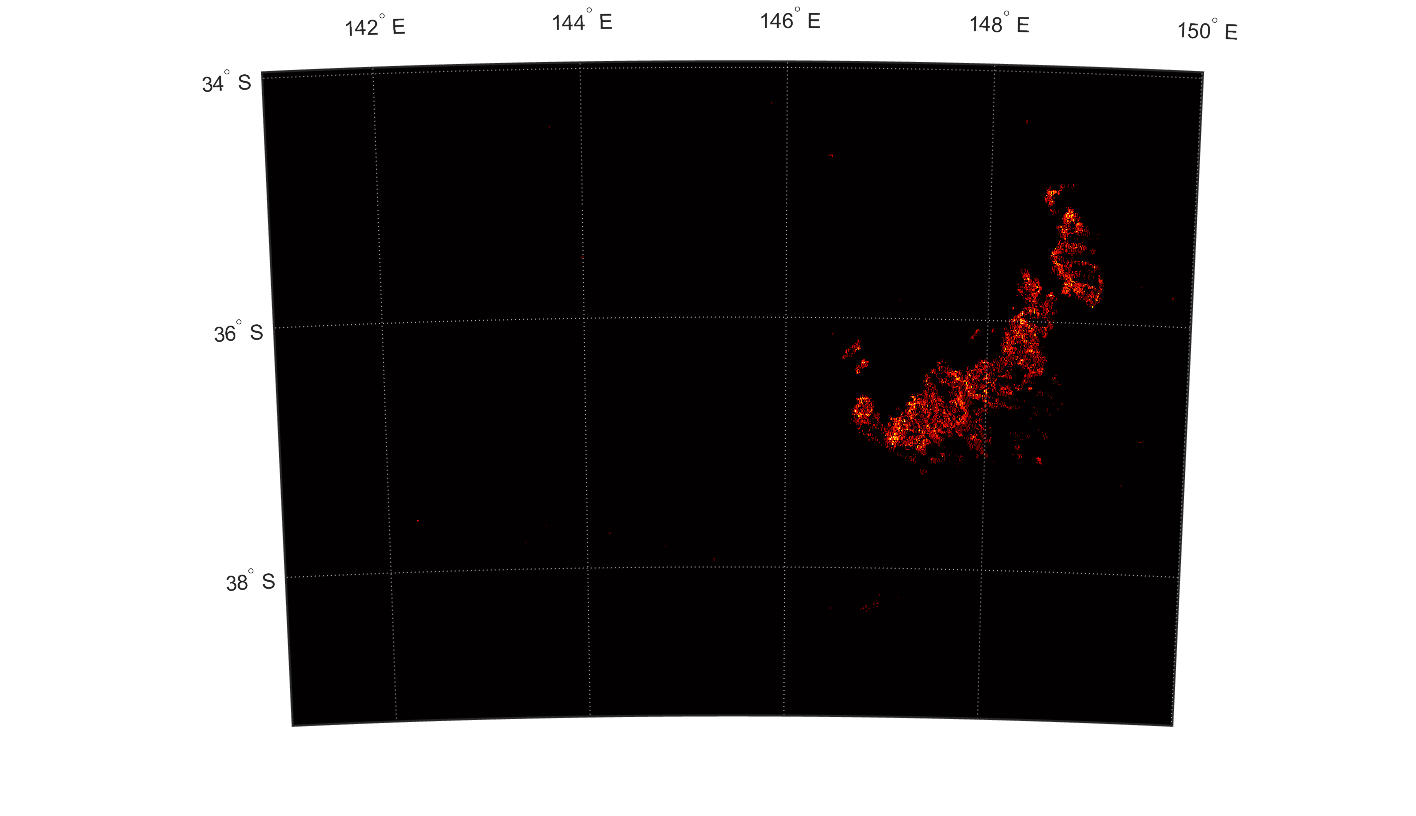
\includegraphics{modis_2003_1_Australia.png}
\caption{}
\end{figure}

\begin{figure}
\centering
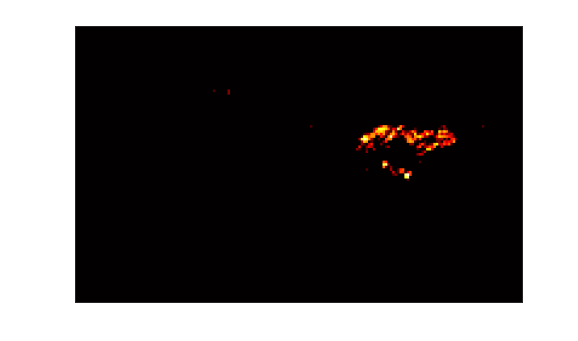
\includegraphics{modis_2003_2_Australia.png}
\caption{}
\end{figure}

\begin{figure}
\centering
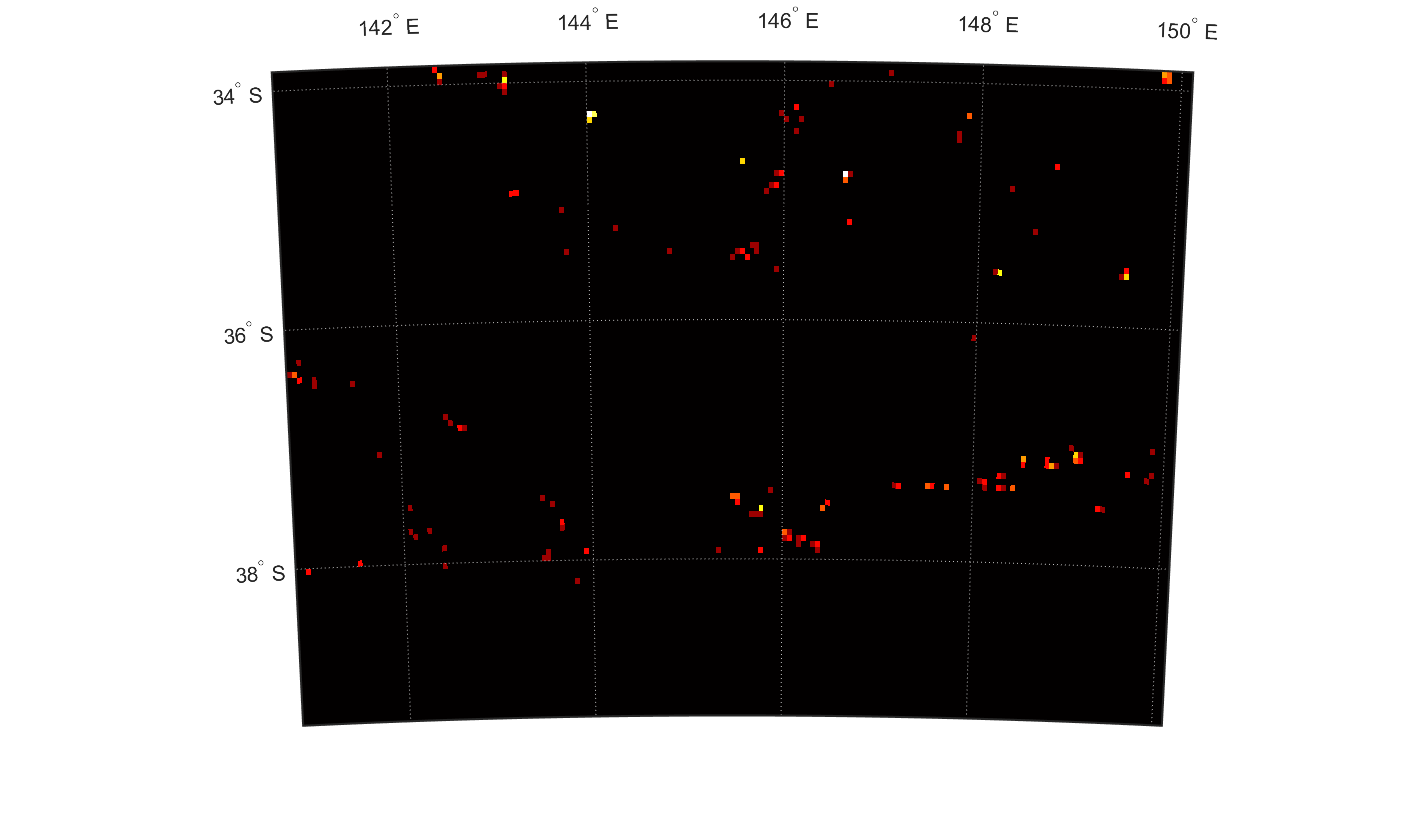
\includegraphics{modis_2003_3_Australia.png}
\caption{}
\end{figure}

\begin{figure}
\centering
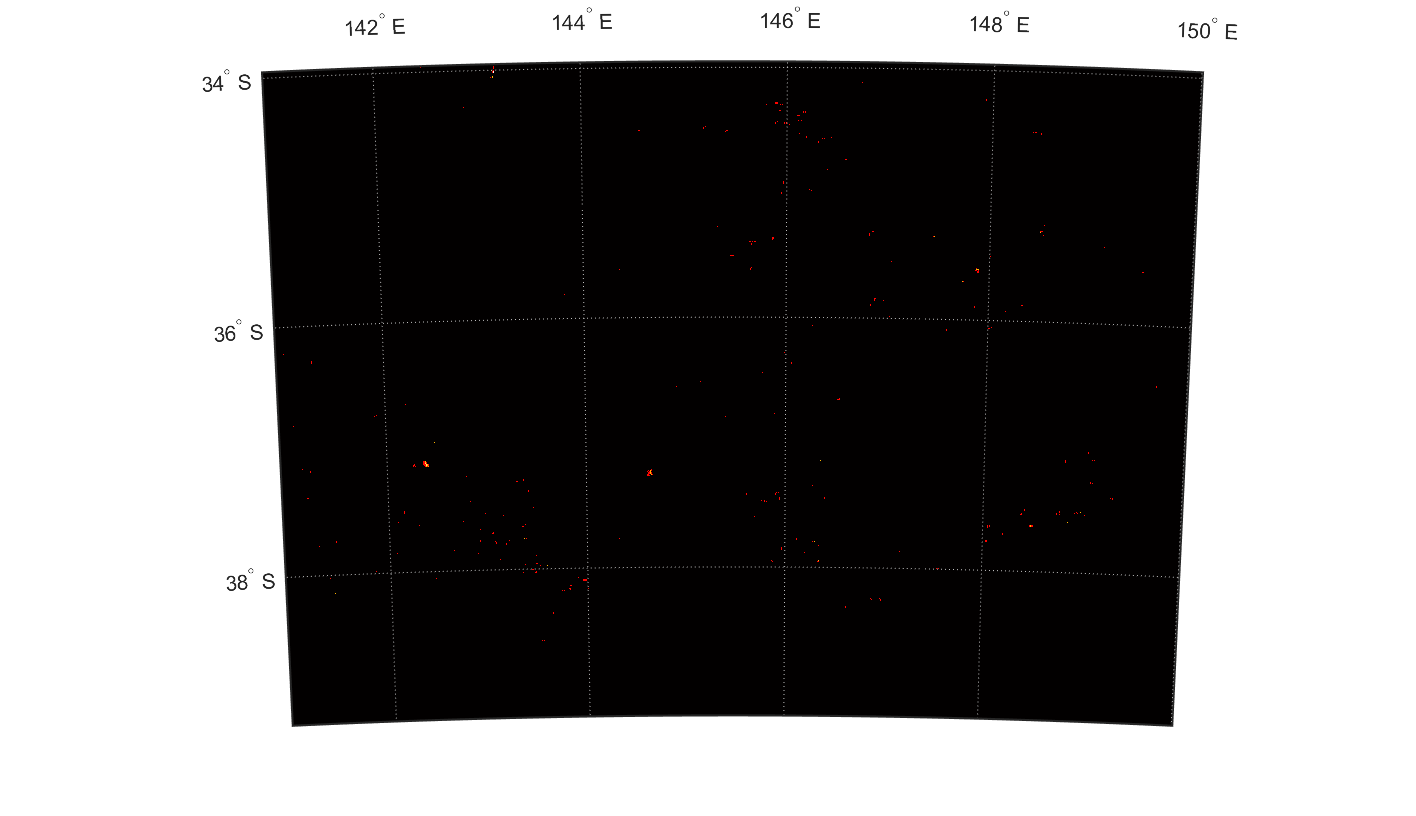
\includegraphics{modis_2003_4_Australia.png}
\caption{}
\end{figure}

\begin{figure}
\centering
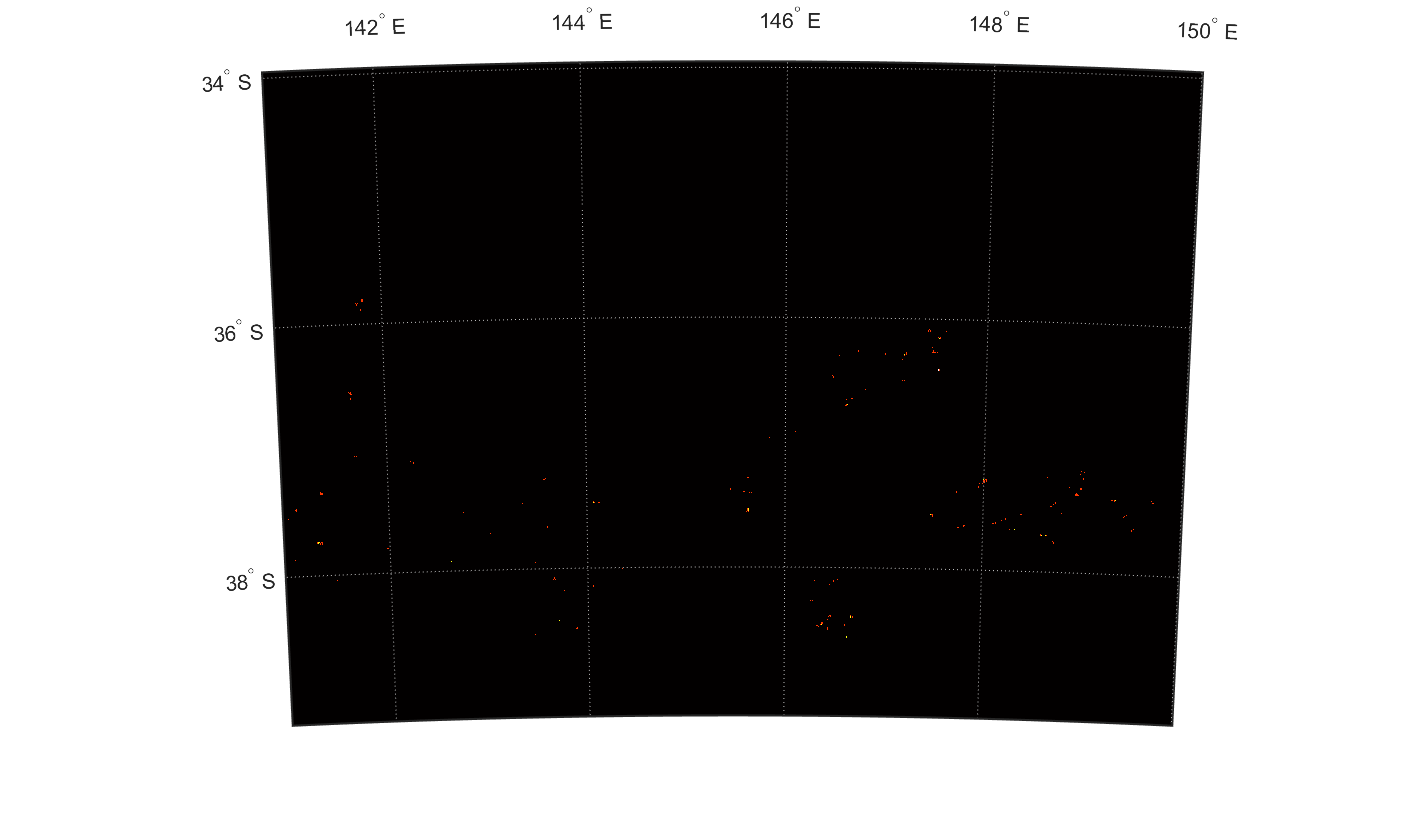
\includegraphics{modis_2003_5_Australia.png}
\caption{}
\end{figure}

\begin{figure}
\centering
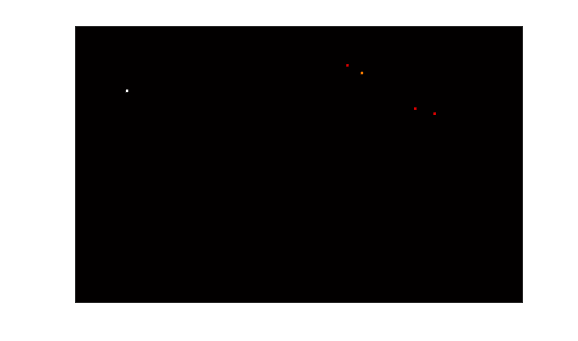
\includegraphics{modis_2003_6_Australia.png}
\caption{}
\end{figure}

\begin{figure}
\centering
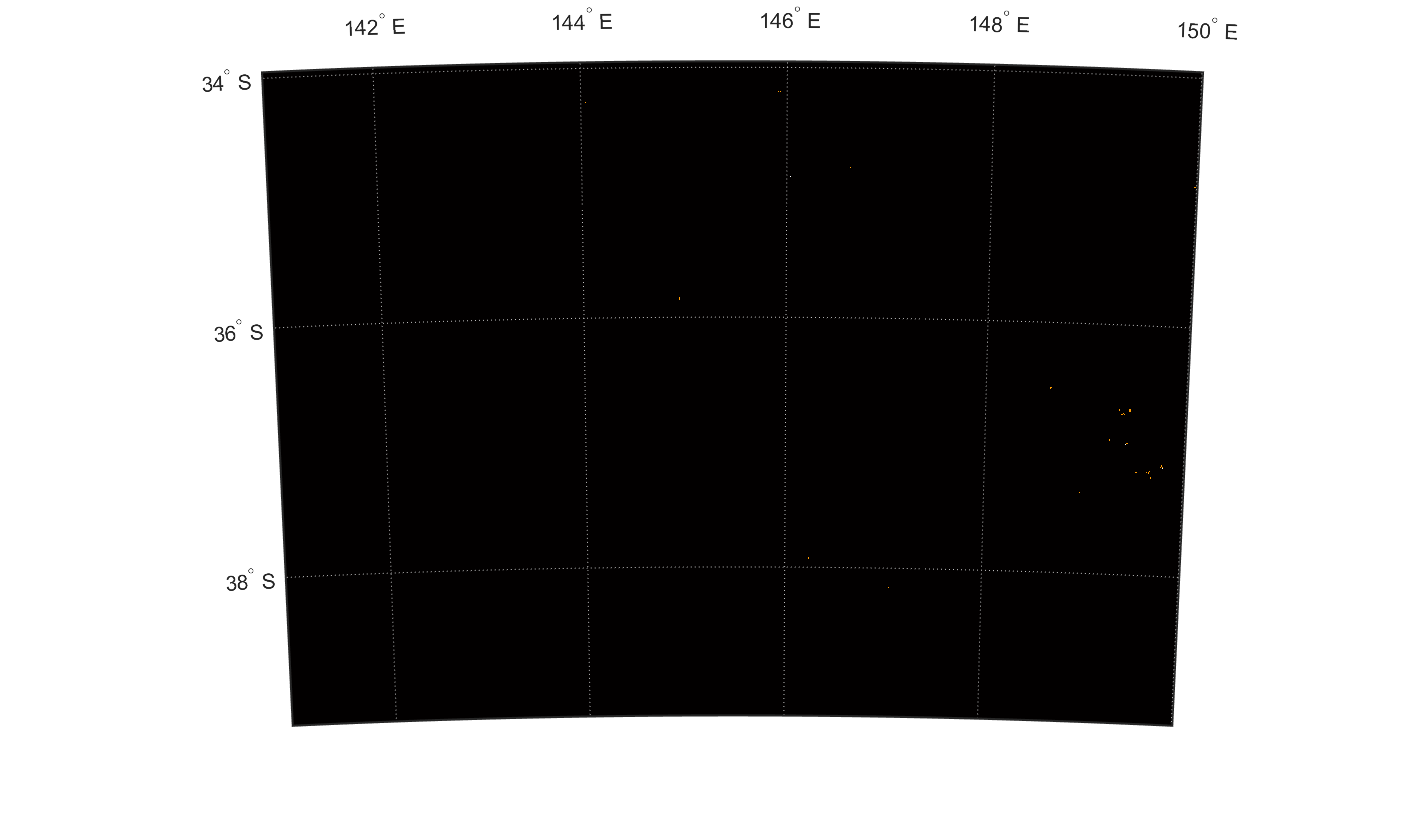
\includegraphics{modis_2003_7_Australia.png}
\caption{}
\end{figure}

\begin{figure}
\centering
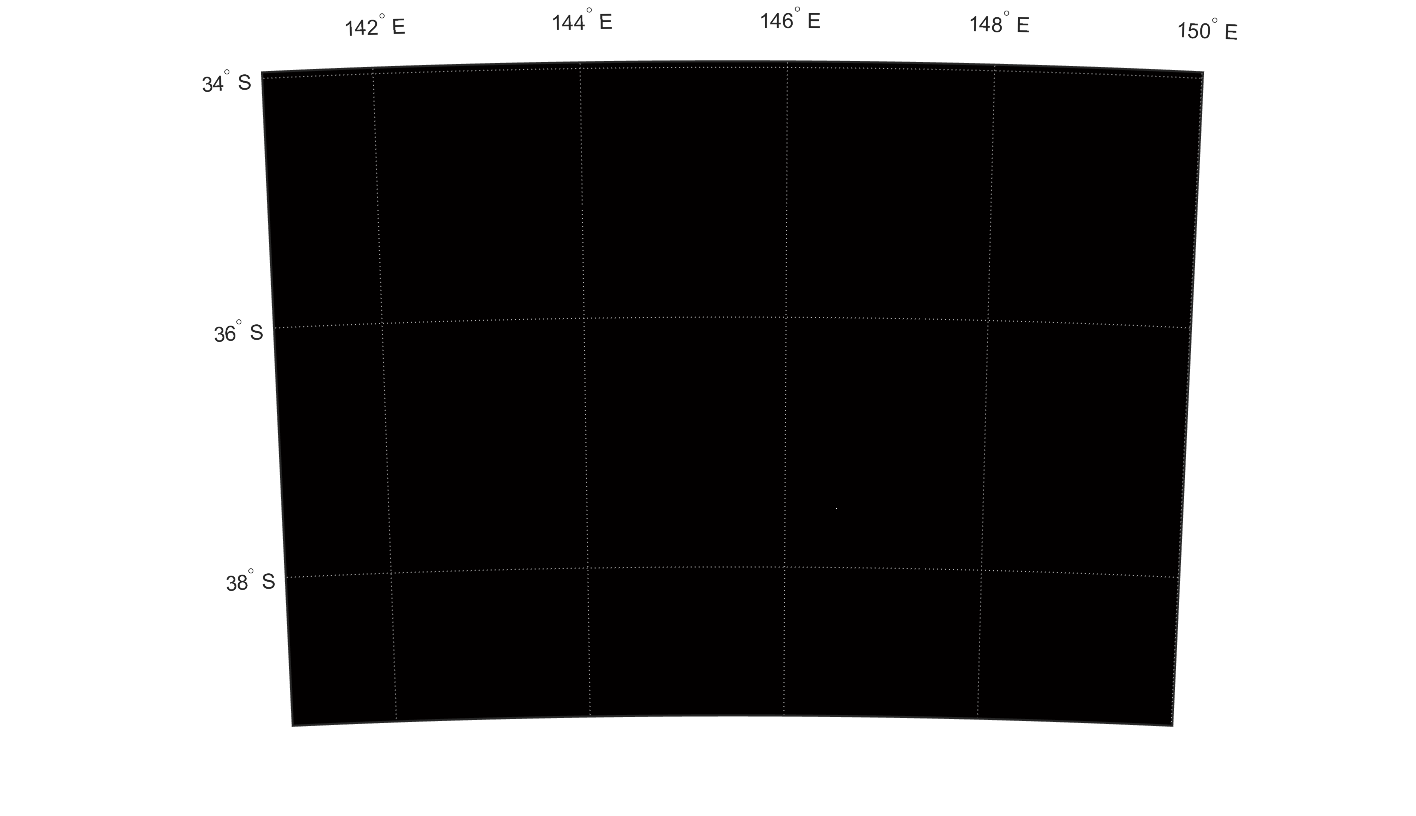
\includegraphics{modis_2003_8_Australia.png}
\caption{}
\end{figure}

\begin{figure}
\centering
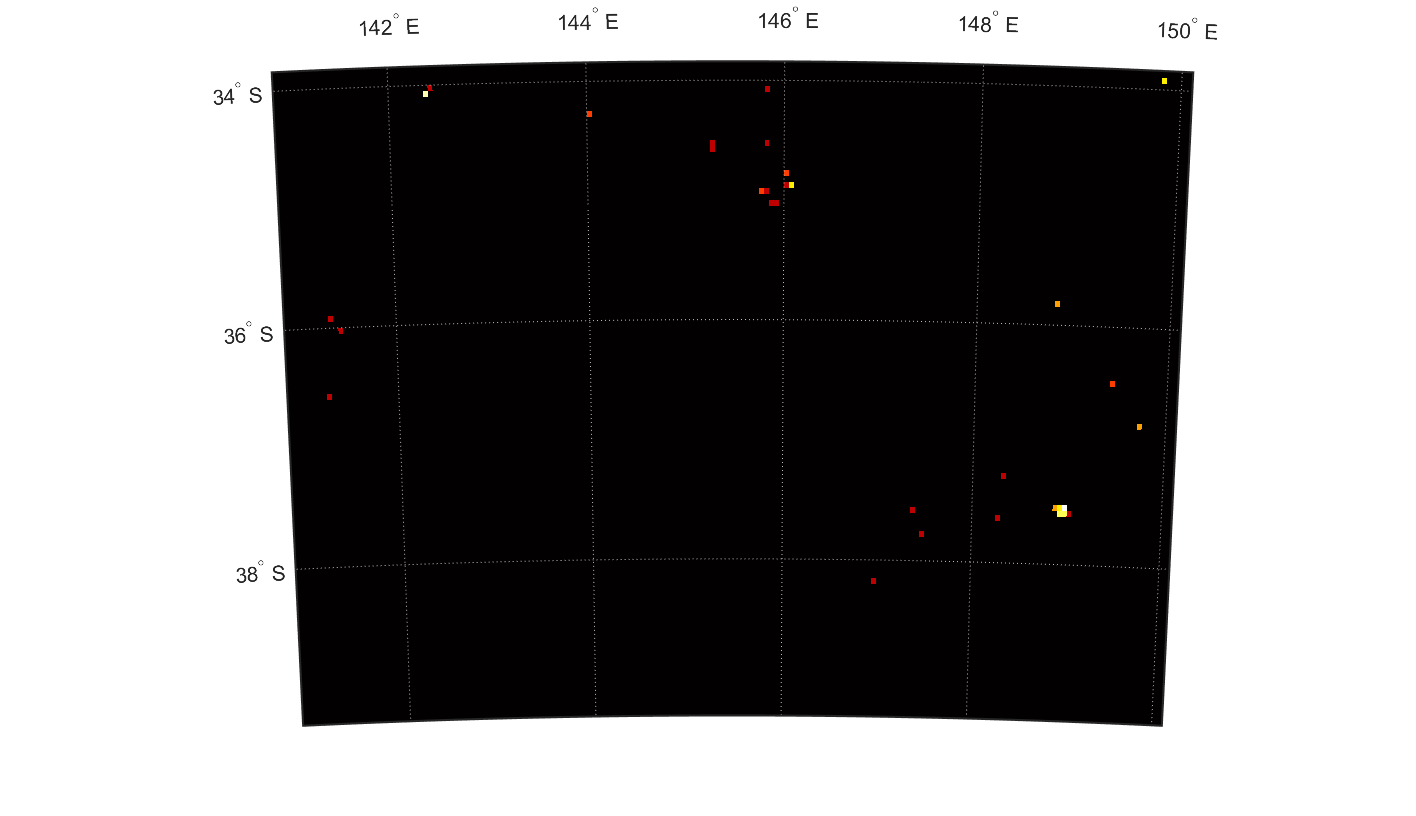
\includegraphics{modis_2003_9_Australia.png}
\caption{}
\end{figure}

\begin{figure}
\centering
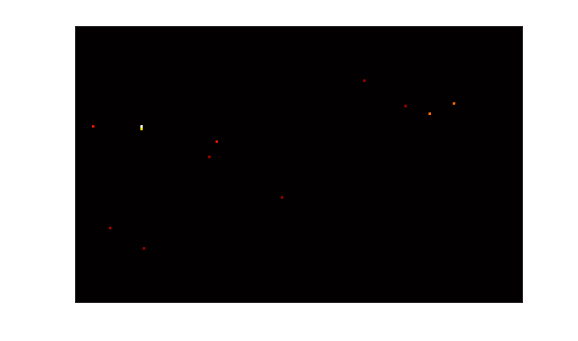
\includegraphics{modis_2003_10_Australia.png}
\caption{}
\end{figure}

\begin{figure}
\centering
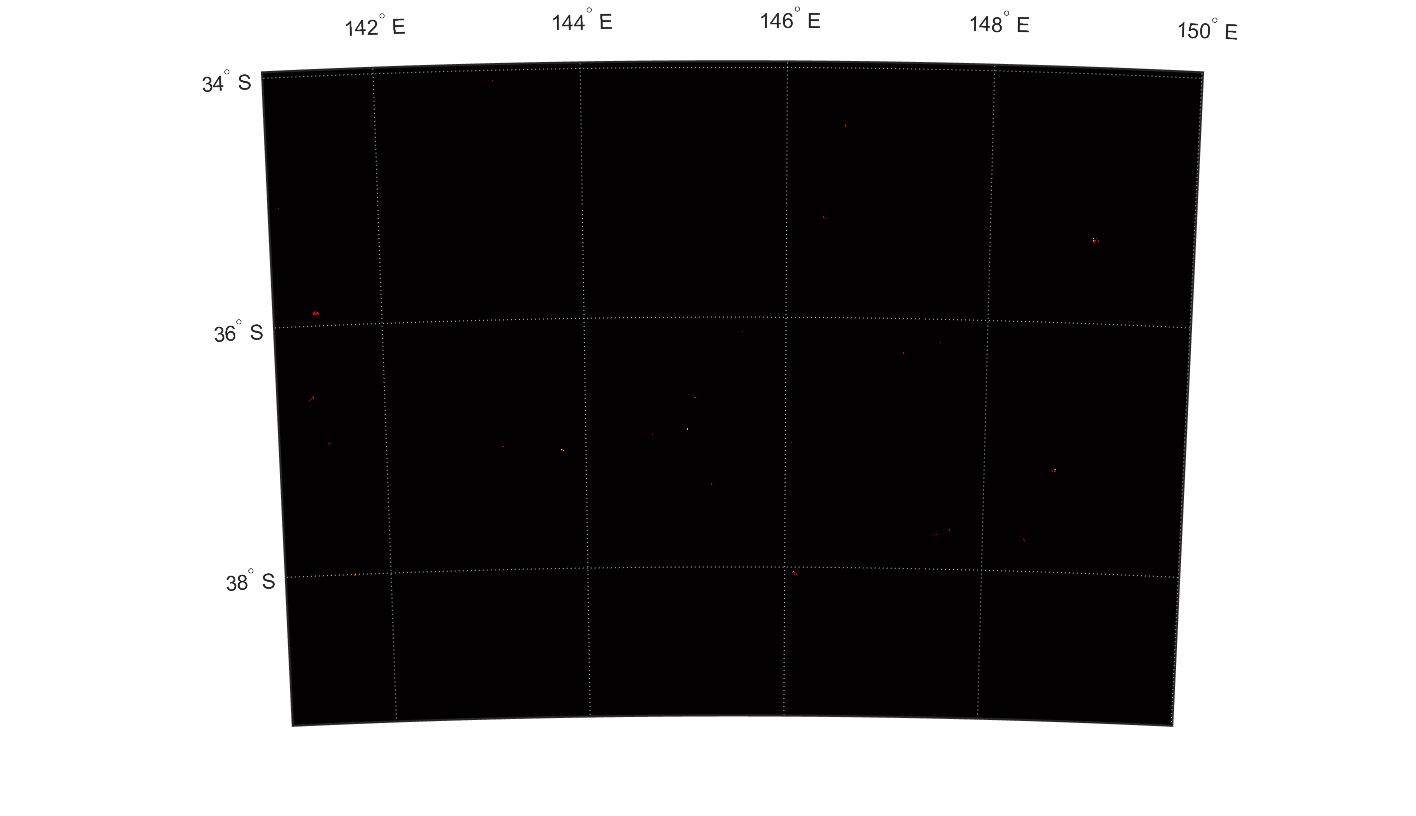
\includegraphics{modis_2003_11_Australia.png}
\caption{}
\end{figure}

\begin{figure}
\centering
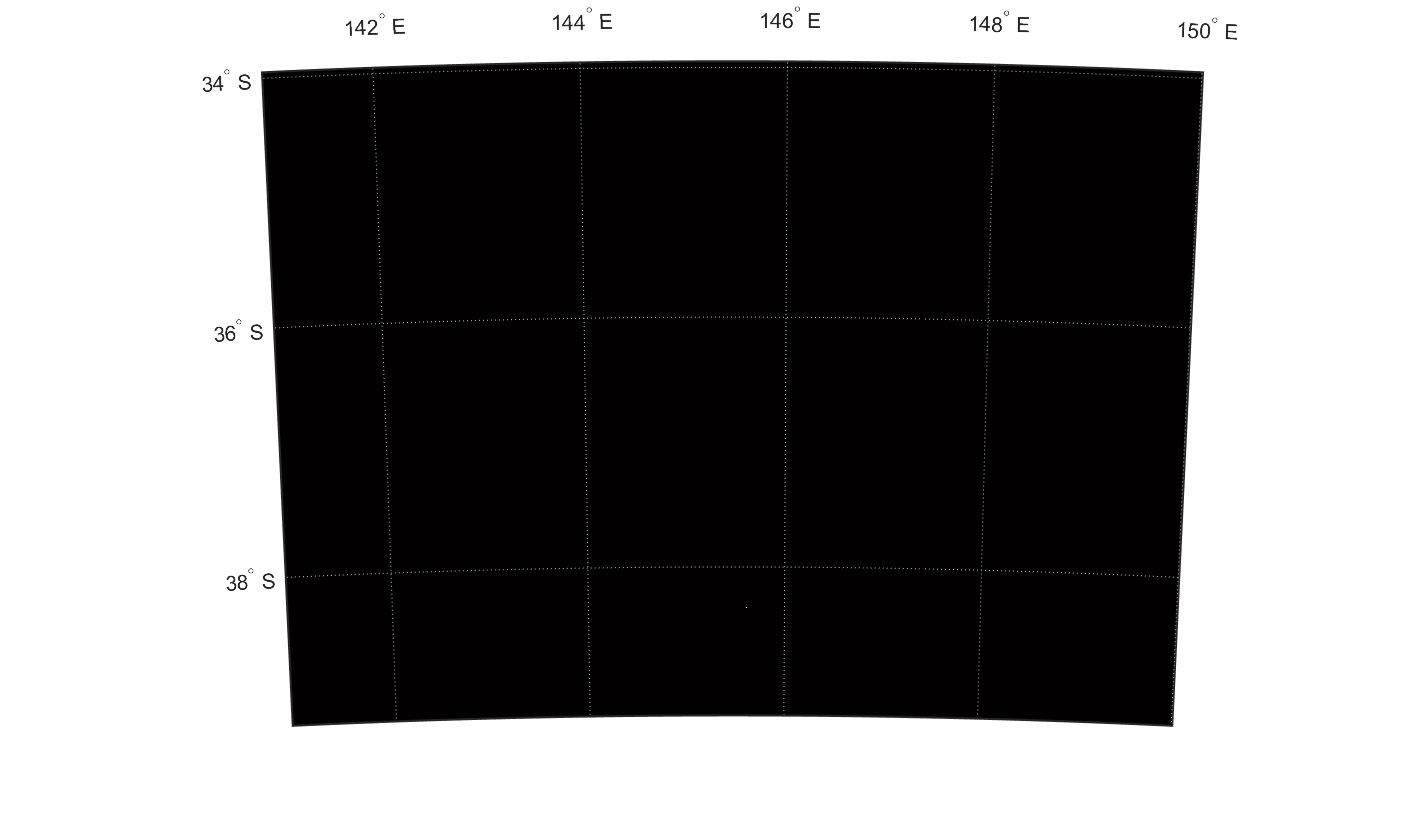
\includegraphics{modis_2003_12_Australia.png}
\caption{}
\end{figure}

The RGB channel values in the picture are given by the following
formula:

\begin{equation}
R_{x,y}=\left\{
\begin{array}{lr}
\left \lfloor 255\frac{3\root4\of{{heat}_{x,y}}}{\max(\root4\of {heat})} \right \rfloor & \root4\of{{heat}_{x,y}}<\frac{1}{3}\max(\root4\of {heat})  \\  
255 & \root4\of{{heat}_{x,y}}\ge\frac{1}{3}\max(\root4\of {heat})
\end{array}  
\right.
\end{equation}

\begin{equation}
G_{x,y}=\left\{
\begin{array}{lr}
0&\root4\of{{heat}_{x,y}}\le\frac{1}{3}\max(\root4\of {heat})\\
\left \lfloor 255\big(\frac{3\root4\of{{heat}_{x,y}}}{\max(\root4\of {heat})}-1\big) \right \rfloor&\frac{1}{3}\max(\root4\of {heat})<\root4\of{{heat}_{x,y}}<\frac{2}{3}\max(\root4\of {heat})  \\  
255&\root4\of{{heat}_{x,y}}\ge\frac{2}{3}\max(\root4\of {heat})
\end{array}  
\right.
\end{equation}

\begin{equation}
B_{x,y}=\left\{
\begin{array}{lr}
0&\root4\of{{heat}_{x,y}}<\frac{2}{3}\max(\root4\of {heat})\\
\left \lfloor 255\big(\frac{3\root4\of{{heat}_{x,y}}}{\max(\root4\of {heat})}-2\big) \right \rfloor&\root4\of{{heat}_{x,y}}\ge\frac{2}{3}\max(\root4\of {heat})  
\end{array}  
\right.
\end{equation}

\hypertarget{time-series-construction}{%
\subsubsection{Time series
construction}\label{time-series-construction}}

\hypertarget{convlstm}{%
\subsubsection{ConvLSTM}\label{convlstm}}

Time series data prediction refers to learning past time series and
predicting future changes. Traditional Neural networks cannot solve the
problem of time-axis variation, so RNN (Recurrent Neural network) is
developed (Jordan et al., 1997).

However, due to the poor performance of classical RNN in extracting long
time series information and the limited time series information
extracted, Hochreiter developed LSTM network model (Hochreiter et
al.,1997). In classical RNN, gates structure is added to selectively add
and delete the past timing information, and input gate, output gate and
forgetting gate are added to control the input and output of data of
this unit (an LSTM cell is a basic unit) and the increase and decrease
of the output information of the previous unit respectively. The LSTM
formula is expressed as follows:

\begin{equation}
\mathbf{i}_t=\sigma(\mathbf{W}_{xi}\mathbf{X}_{t}+\mathbf{W}_{hi}\mathbf{H}_{t-1}+\mathbf{W}_{ci}\circ\mathbf{C}_{t-1}+b_i)
\end{equation}

\begin{equation}
\mathbf{f}_t=\sigma(\mathbf{W}_{xf}\mathbf{X}_{t}+\mathbf{W}_{hf}\mathbf{H}_{t-1}+\mathbf{W}_{cf}\circ\mathbf{C}_{t-1}+b_f) 
\end{equation}

\begin{equation}
\mathbf{C}_t=\mathbf{f}_{t}\circ\mathbf{C}_{t-1}+\mathbf{i}_t\circ\tanh(\mathbf{W}_{xc}\mathbf{X}_{t}+\mathbf{W}_{hc}\mathbf{H}_{t-1}+b_c)
\end{equation}

\begin{equation}
\mathbf{o}_t=\sigma(\mathbf{W}_{xo}\mathbf{X}_{t}+\mathbf{W}_{ho}\mathbf{H}_{t-1}+\mathbf{W}_{co}\circ\mathbf{C}_{t-1}+b_o)
\end{equation}

ConvLSTM is a variant of LSTM proposed on the basis of LSTM. It replaces
the fully connected state between the input layer and the hidden layer
and between the hidden layer and the hidden layer of LSTM with the
convolution connection, which makes full use of the spatial information
that LSTM cannot. LSTM needs to transform image data into
one-dimensional vector when processing image data, and cannot process
spatial structure information of original image data. Compared with LSTM
model,Conv LSTM can better extract spatial and temporal structure
information from time series images. ConvLSTM model formula is expressed
as follows:

\begin{equation}
\mathbf{i}_t=\sigma(\mathbf{W}_{xi}*\mathbf{X}_{t}+\mathbf{W}_{hi}*\mathbf{H}_{t-1}+\mathbf{W}_{ci}\circ\mathbf{C}_{t-1}+b_i)
\end{equation}

\begin{equation}
\mathbf{f}_t=\sigma(\mathbf{W}_{xf}*\mathbf{X}_{t}+\mathbf{W}_{hf}*\mathbf{H}_{t-1}+\mathbf{W}_{cf}\circ\mathbf{C}_{t-1}+b_f) 
\end{equation}

\begin{equation}
\mathbf{C}_t=\mathbf{f}_{t}\circ\mathbf{C}_{t-1}+\mathbf{i}_t\circ\tanh(\mathbf{W}_{xc}*\mathbf{X}_{t}+\mathbf{W}_{hc}*\mathbf{H}_{t-1}+b_c)
\end{equation}

\begin{equation}
\mathbf{o}_t=\sigma(\mathbf{W}_{xo}*\mathbf{X}_{t}+\mathbf{W}_{ho}*\mathbf{H}_{t-1}+\mathbf{W}_{co}\circ\mathbf{C}_{t-1}+b_o)
\end{equation}

The symbol meaning in the formula is the same as that in LSTM. The full
connection of input variables is replaced by convolution operation.
According to the internal structure of ConvLSTM in figure, it can be
seen that input gate, output gate and forgetting gate all carry out
convolution operation for input and hidden layer.

\begin{figure}
\centering
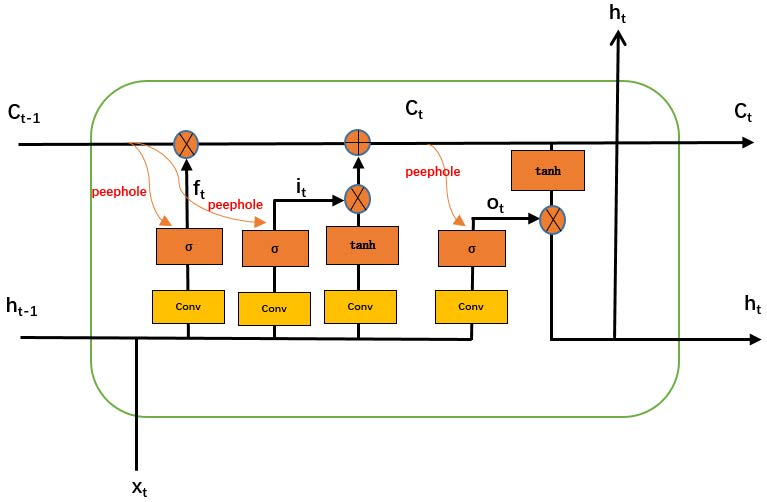
\includegraphics{Structure_of_ConvLSTM_Cell.jpg}
\caption{}
\end{figure}

\(\mathbf{W}_{ci}\circ\mathbf{C}_{t-1}\),
\(\mathbf{W}_{cf}\circ\mathbf{C}_{t-1}\) and
\(\mathbf{W}_{co}\circ\mathbf{C}_{t-1}\) in the formula indicate
that the input, output and forgetting gates are connected to the
Peephole(Gers et al., 2000) of the previous cellular state. As shown in
the figure, the Peephole connection adds cell state information to each
gate. Since the unit may have a door state of 0, which results in a lack
of important information, adding the Peephole operation can improve this
shortcoming.

Based on the deep learning framework Pytorch, the ConvLSTM is
constructed using Python language, and the experimental equipment
environment is NVIDIA GeForce GTX1080 GPU.

\hypertarget{model-fitting}{%
\subsubsection{Model Fitting}\label{model-fitting}}

\end{document}
